Building such a platform from scratch can be quite expensive while there are many parts that can be integrated together. Integration of different parts together can reduce the price significantly. There are two main parts of our solution. There is a drone and its controller on one side and the VR headset with sensors on the other side. They are connected together through the Internet, so the latency greatly depends on the quality of your connection. That is why we decided to use 360\degree camera instead of a traditional drone camera placed on gimbal. We can transfer 360\degree video with large compression of areas, which are out of viewers viewport. This can be done by mapping image onto the pyramids and therefore reduce the amount of transferred data by 80\%\cite{facebook2016videoencoding}.

\subsection{Drone and controller}
For building a prototype it is easier to start with some kind of a drone kit. Therefore, we chose quadrocopter with mounts for the other hardware and camera\footnote{\url{http://www.robotshop.com/en/lynxmotion-hquad500-drone-base-combo-kit-quadrino-nano-controller.html}}. It is definitely more expensive than having a drone with all hardware integrated in one body, but for the purpose of future tweaking of our idea, the kit is better. 

Chosen controller contains GPS, accelerometer, gyroscope and accelerometer and it would be possible to pair this controller with autopilot module\footnote{\url{http://www.robotshop.com/en/navio2-autopilot-kit-raspberry-pi-2-3.html}}. Autopilot module is optional, but for our experiments it would be necessary. During the experiments we want to find out, which way of controlling drone is easier for the users. If there is big latency in communication, the autopilot can be the way to go. It can be also connected together with Viooa camera and drone, then can provide features such as tripod mode, follow me mode or fly around.

For the success of this solution is crucial battery life. Therefore, we have to integrate battery that allows drone at least 20 minutes of flight. This item can be adjusted as we need, but from the start, we chose battery with 3500 mAh\footnote{\url{http://www.robotshop.com/en/111v-3500mah-30c-lipo-battery.html}}.

\subsection{Camera}
For our solution we decided to use 360\degree$\times$180\degree camera Viooa\footnote{\url{http://www.viooa.com/viooa.html}}. This camera shoots 4k footage and integrates a lot of smart algorithms that can help with controlling the actual drone.

This camera can be mounted to the bottom or the front of the drone and the image from the camera will be streamed over the WiFi to the phone and then over the Internet right to the VR headset.

\subsection{VR headset}
We chose Oculus Rift VR headset\footnote{\url{https://www.oculus.com/rift/}}, which supports all features we need and furthermore it also has touch controls Oculus Touch. Touch controls can be used for fine drone controlling or it can be used by people, who have limited head movements. 

\subsection{Software}
To transfer data between the drone and a viewer we have to implement software, which will be able to operate with high amount of data. To compress the data, we want to use Facebook's implementation of 360\degree video, that maps the original footage to the multiple pyramids and saves a huge amount of data\cite{facebook2016videoencoding}. We also have to implement a system, that deals with the latency of the connection and it can be quite challenging. Other solutions, such as DJI Goggles, are dealing with few kilometers of distance (at maximum) and they keep latency at 100ms only when the drone is on sight.

The actual implementation of client and server software will be done upon a larger discussion. Current proposed solution can serve as a framework for further work.

\subsection{Other requirements}
The most crucial requirement for pleasant experience is good internet connection between the drone and the viewer. Thanks to the modern mobile technologies, we are now able to transfer large amount of data over the mobile networks with a decent latency. Our architecture proposal can be seen on figure \ref{fig:connection}.

\begin{figure}[h!]
    \centering
    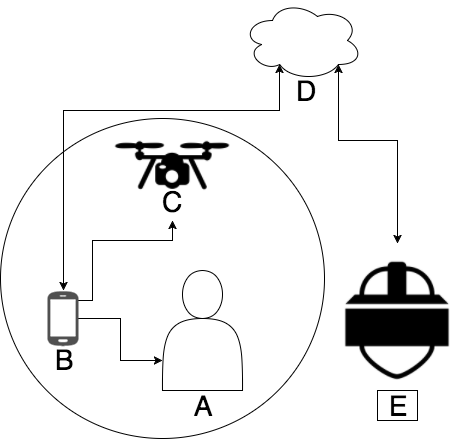
\includegraphics[width=0.40\textwidth]{img/connectiondiagram}
    \caption[]{Diagram of system architecture:\newline A - Traveller, B - Mobile device, C - Drone,\newline D - Clouse service, E - Pilot with controlling headset}
    \label{fig:connection}
\end{figure}

\subsection{Price}
Price is probably something, what can be reduced with further development of the product and integrate all the components in the one body. Price can be split between drone and VR headset, because many people can already have some kind of compatible headset they can use. Detailed prices of the components are shown in table \ref{estimatedprice}.

\bgroup
\def\arraystretch{1.5}
\begin{table}[h!]
\centering
\begin{tabular}{p{4}p{2.5cm}}
\textbf{Item}                                                          & \textbf{Estimated price (USD)} \\ \hline
\multicolumn{2}{l}{\textit{Drone}}                                                             \\ \hline
\multicolumn{1}{l|}{Drone body + controller}                  & 520 (+250 for autopilot)                   \\
\multicolumn{1}{l|}{Viooa 360\degree camera (or alternative)} & $\sim$700             \\
\multicolumn{1}{l|}{Remote control}                           & 130                   \\
\multicolumn{1}{l|}{Battery \& other drone modules}       & 100                   \\ \hline\hline
\multicolumn{2}{l}{\textit{Viewer}}                                                            \\ \hline
\multicolumn{1}{l|}{Oculus Rift}                              & 600                   \\ \hline\hline
\textbf{Total}                                                         & \textbf{2300}                  \\ \hline
\end{tabular}
\caption{Estimated price of prototype}
\label{estimatedprice}
\end{table}
\egroup
